\documentclass[11pt,a4paper]{article}
\usepackage[margin=2.2cm]{geometry}
\usepackage{graphicx}
\usepackage{booktabs}
\usepackage{xcolor}
\usepackage{hyperref}
\hypersetup{colorlinks=true,linkcolor=blue!50!black,urlcolor=blue!50!black}
\definecolor{accent}{RGB}{20,70,140}
\setlength{\parskip}{4pt}
\setlength{\parindent}{0pt}
\newcommand{\sect}[1]{\section{\textcolor{accent}{#1}}}

\begin{document}

\begin{center}
{\LARGE\bfseries\textcolor{accent}{SPI RTL to GDS Flow}}\\[6pt]
{\large APB3 SPI Master Controller: RTL Design, UVM Verification and SKY130 Physical Design}\\[10pt]
{\bfseries M Kamaraju}\\
\href{https://github.com/MKRAJU-VLSI-HUB/spi-rtl-to-gds-flow}{github.com/MKRAJU-VLSI-HUB/spi-rtl-to-gds-flow}
\quad$\cdot$\quad
\href{https://www.linkedin.com/in/magupallikamaraju/}{linkedin.com/in/magupallikamaraju}
\end{center}

\vspace{4pt}
\begin{center}
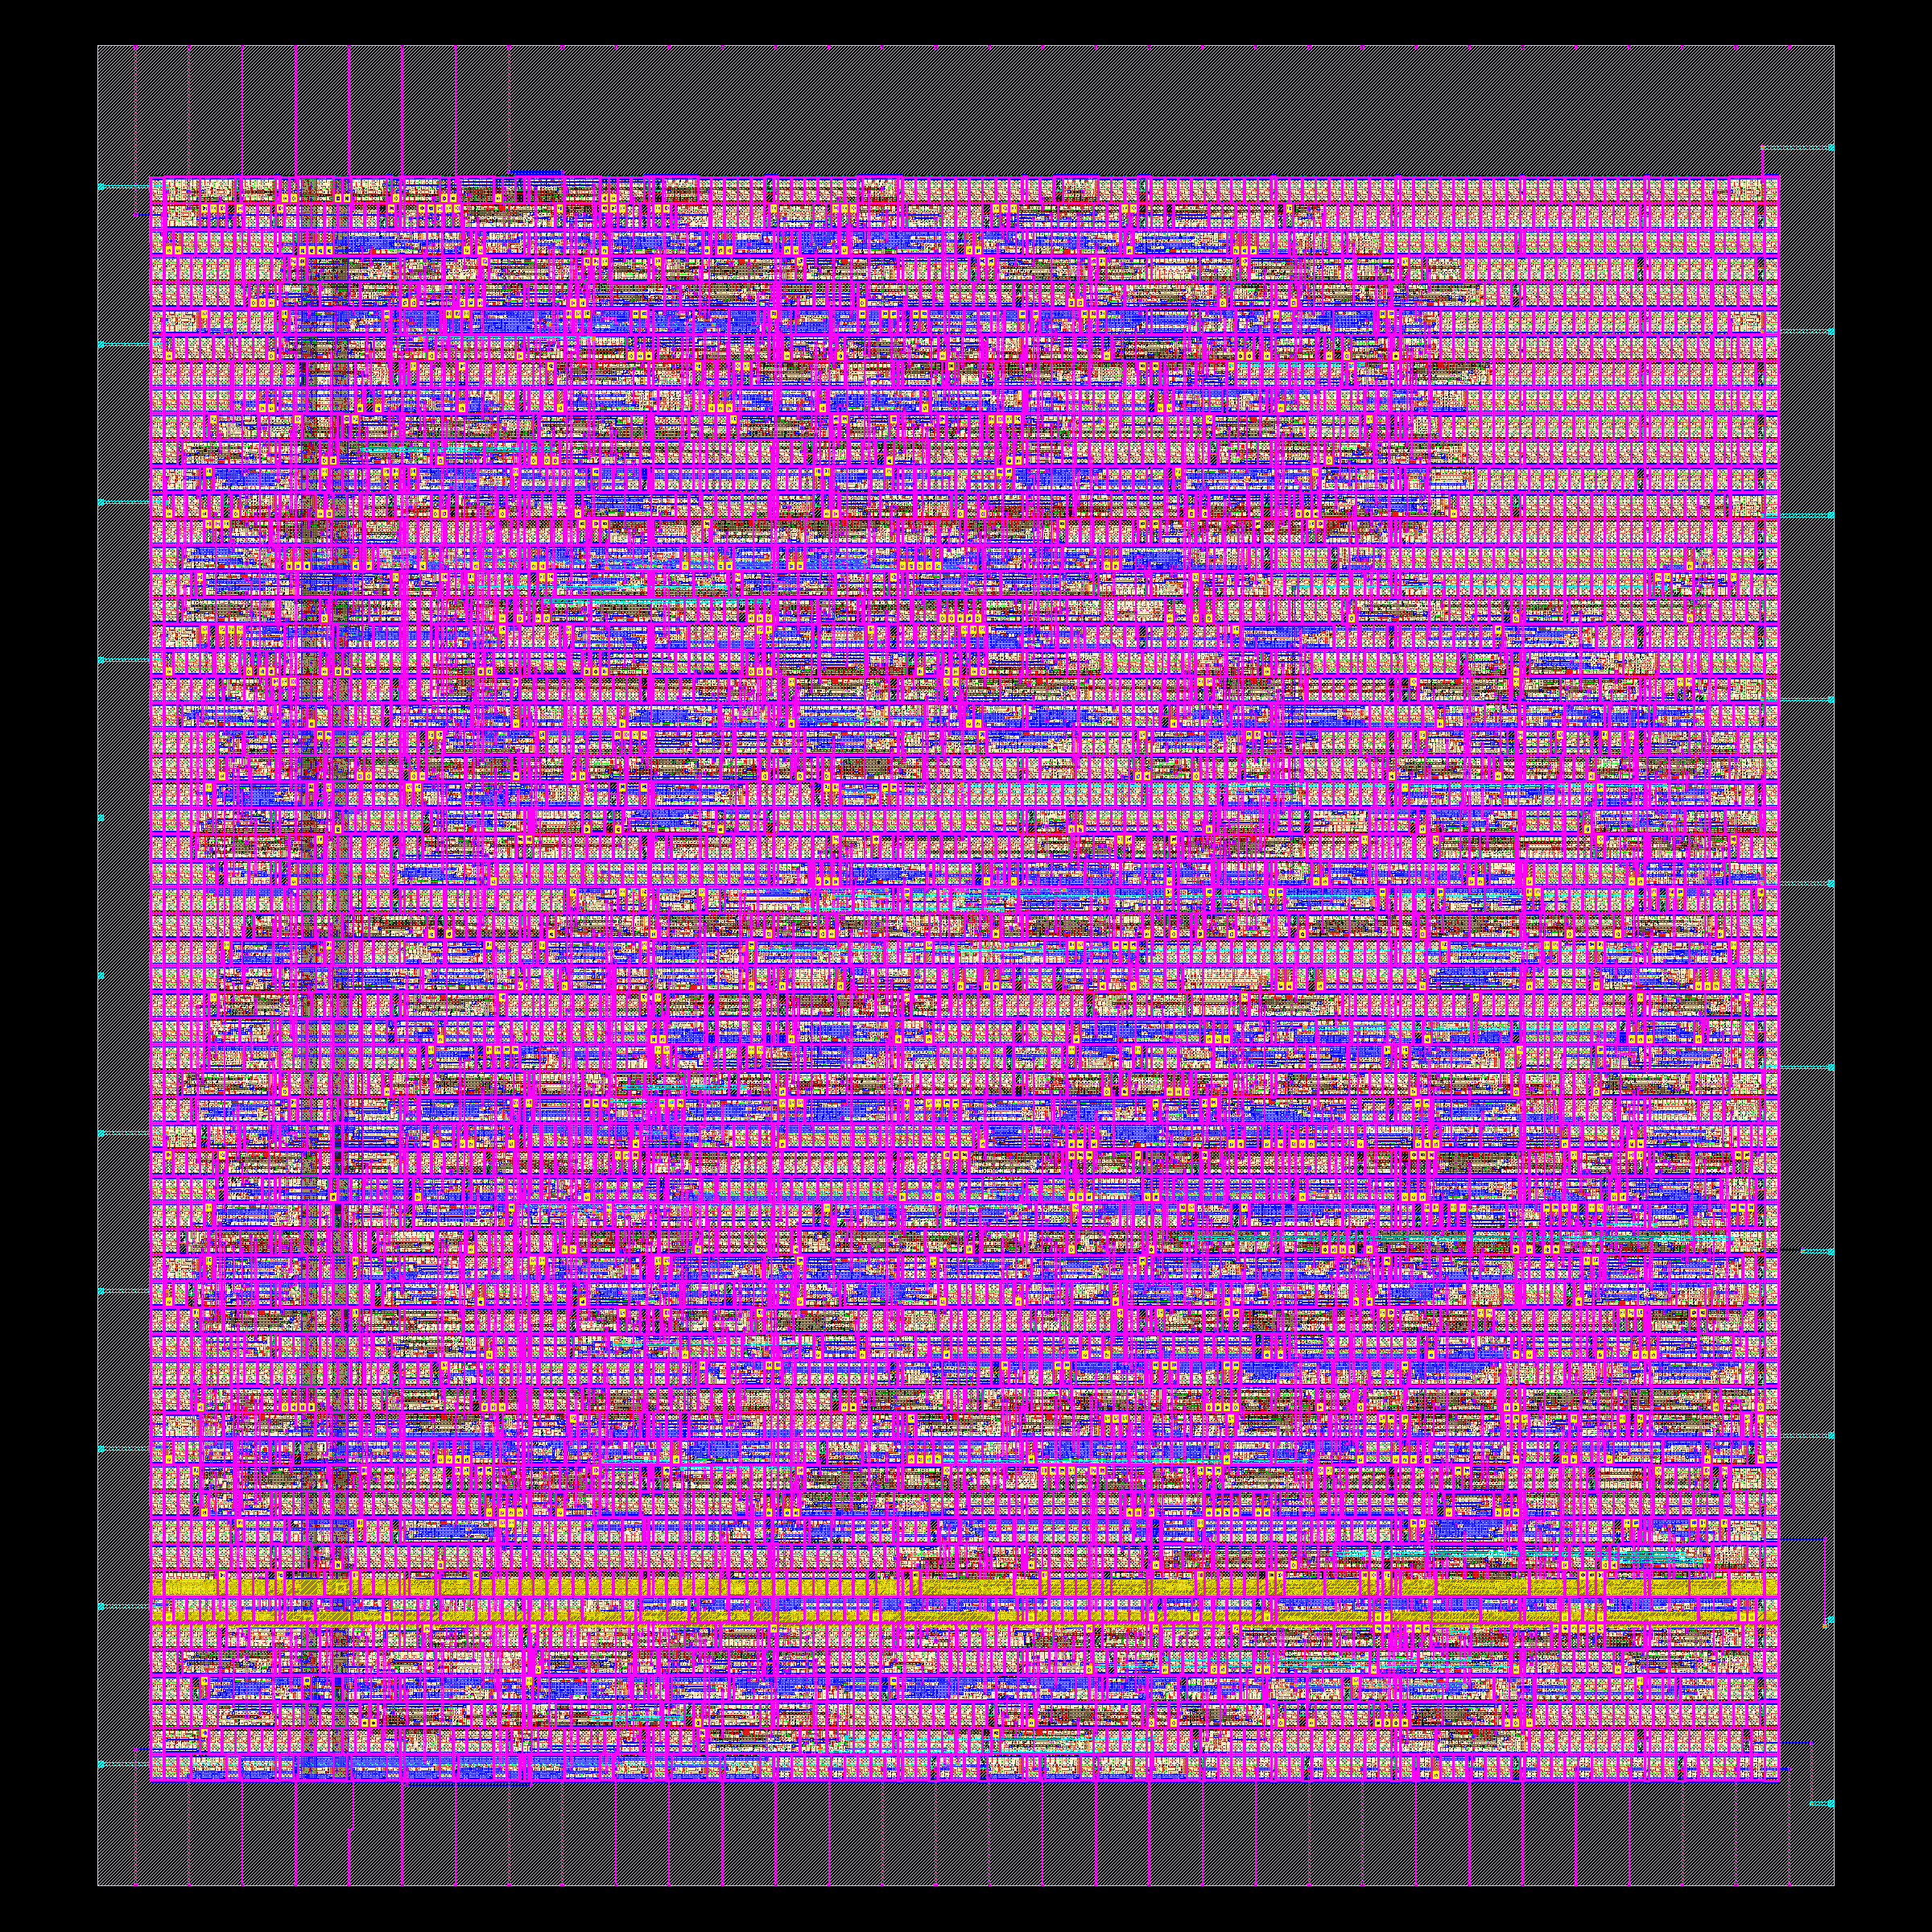
\includegraphics[width=0.58\textwidth]{images/spi_top_layout.png}\\
{\small Final GDSII layout of \texttt{spi\_top} on SkyWater SKY130 (179.7\,$\mu$m $\times$ 190.4\,$\mu$m)}
\end{center}

\sect{Project Summary}
This project takes an SPI master controller with an AMBA APB3 interface through a complete ASIC design flow. The design was written in synthesizable Verilog, verified with a UVM 1.2 environment that uses a reactive SPI slave model, SystemVerilog assertions and code and functional coverage, and implemented from RTL to GDSII on the open SkyWater 130\,nm PDK using OpenLane~2 (Yosys, OpenROAD, Magic, KLayout, Netgen).

\begin{center}
\begin{tabular}{ll}
\toprule
\textbf{Item} & \textbf{Result} \\
\midrule
UVM regression & 10/10 tests pass, 0 mismatches, 0 assertion failures \\
Functional coverage (merged) & 99.80\,\% \\
Code coverage (DUT) & statement 100\,\%, branch 95--100\,\%, condition 93--100\,\% \\
Toggle coverage & 109/109 port and register bits (100\,\%) \\
Signoff frequency & 50\,MHz, met in all 9 PVT/RC corners \\
Setup / hold WNS & +2.57\,ns / +0.11\,ns \\
Die area & 0.034\,mm$^2$ (179.7\,$\mu$m $\times$ 190.4\,$\mu$m) \\
Cells / power & 793 cells (219 flip-flops) / 1.68\,mW \\
DRC / LVS / antenna & 0 violations / clean / 0 \\
\bottomrule
\end{tabular}
\end{center}

\sect{Design Specification}
\begin{itemize}
\item APB3 slave interface: zero wait state, \texttt{PSLVERR} on unmapped addresses.
\item All four SPI modes (CPOL/CPHA), MSB- or LSB-first, 8-bit frames.
\item Programmable clock: $f_{SCLK} = f_{PCLK} / (2\,(CLKDIV+1))$.
\item 8-deep TX and RX FIFOs, with back-to-back bytes inside one chip-select frame.
\item Half-SCLK chip-select setup and hold time; registered, glitch-free SCLK and MOSI.
\item Four chip selects with automatic (per burst) or manual (software) control.
\item Interrupts: RX available, TX empty, transfer done, RX overrun, TX overflow (sticky bits are write-1-to-clear); internal loopback.
\end{itemize}

\begin{center}
\small
\begin{tabular}{lllp{9.2cm}}
\toprule
\textbf{Off.} & \textbf{Name} & \textbf{Acc.} & \textbf{Description}\\
\midrule
0x00 & TXDATA & W & push byte into TX FIFO \\
0x04 & RXDATA & R & pop byte from RX FIFO \\
0x08 & CTRL & RW & EN, CPOL, CPHA, LSB\_FIRST, LOOPBACK, CS\_MANUAL \\
0x0C & CLKDIV & RW & 8-bit SCLK divider (reset 4) \\
0x10 & STATUS & R & FIFO full/empty, BUSY, TX and RX FIFO levels \\
0x14 & IER & RW & interrupt enables \\
0x18 & ISR & R/W1C & RX\_AVAIL, TX\_EMPTY, DONE, RX\_OVERRUN, TX\_OVERFLOW \\
0x1C & CSREG & RW & CS\_SEL[1:0], CS\_ASSERT (manual mode) \\
\bottomrule
\end{tabular}
\end{center}

\textbf{RTL hierarchy:} \texttt{spi\_top} contains \texttt{spi\_regs} (APB registers and interrupt logic), two \texttt{spi\_fifo} instances, and \texttt{spi\_master}, the shift engine with IDLE, LEAD, XFER and TRAIL states. The engine produces 16 SCLK edges per byte, sampling on leading or trailing edges according to CPHA, and latches its configuration at the start of every byte. Chip-select decoding is one-hot, and no slave is selected in loopback mode.

\sect{UVM Verification Environment}
\begin{itemize}
\item \textbf{APB agent:} sequencer, APB3 master driver and monitor.
\item \textbf{SPI agent:} a reactive slave model that returns a random byte per transfer, following the live CPHA and bit order, plus a bus monitor that decodes MOSI and MISO on the CPHA-selected edges for the active chip select.
\item \textbf{Scoreboard:} MOSI path (APB writes to bytes on MOSI), MISO path (slave bytes to APB reads), loopback path, chip-select index, TX overflow (via a white-box full flag), RX overrun model, sticky ISR model with W1C, register mirrors, and PSLVERR decoding.
\end{itemize}

\subsection*{Assertions (SVA, bound into the DUT)}
36 concurrent assertions and 9 cover properties check APB protocol rules, FIFO integrity, SCLK at the CPOL idle level, SCLK toggling only during a transfer, chip select held for every transfer, one-hot and correctly decoded \texttt{ss\_n}, no slave selected in loopback, exactly 16 SCLK edges per byte, DONE pulse semantics, overrun/overflow/done flag setting, sticky bits cleared only by W1C, \texttt{irq} $=$ OR(ISR \& IER), and reset values.

\subsection*{Regression results (Vivado 2024.2 XSIM)}
\begin{center}
\small
\begin{tabular}{lp{8.6cm}c}
\toprule
\textbf{Test} & \textbf{Scenario} & \textbf{Result}\\
\midrule
spi\_smoke\_test & mode 0 basic transfers & PASS\\
spi\_reg\_test & reset values, R/W patterns, RO registers, PSLVERR & PASS\\
spi\_mode\_test & all 4 modes $\times$ MSB/LSB first & PASS\\
spi\_clkdiv\_test & CLKDIV from 0 to 255 & PASS\\
spi\_cs\_test & each chip select, automatic and manual frames & PASS\\
spi\_overflow\_test & 11 writes into an 8-deep TX FIFO & PASS\\
spi\_overrun\_test & 11 received bytes into an 8-deep RX FIFO & PASS\\
spi\_loopback\_test & internal loopback, random modes & PASS\\
spi\_irq\_test & each interrupt source: set, mask, clear & PASS\\
spi\_random\_test & constrained-random mix incl. manual CS frames & PASS\\
\bottomrule
\end{tabular}
\end{center}

\subsection*{Coverage}
\begin{center}
\small
\begin{tabular}{lr@{\hspace{1.2cm}}lrrr}
\toprule
\textbf{Covergroup} & \textbf{Score} & \textbf{Module} & \textbf{Stmt} & \textbf{Branch} & \textbf{Cond}\\
\midrule
cg\_xfer (mode/order/CS) & 100\,\% & spi\_regs & 100\,\% & 100\,\% & 100\,\% \\
cg\_data (MOSI/MISO) & 100\,\% & spi\_master & 100\,\% & 95\,\% & 100\,\% \\
cg\_div & 100\,\% & spi\_fifo & 100\,\% & 100\,\% & 92.86\,\% \\
cg\_apb & 98.61\,\% & spi\_top & -- & 100\,\% & -- \\
cg\_isr, cg\_status, cg\_ctrl & 100\,\% & & & & \\
\midrule
\textbf{Merged total} & \textbf{99.80\,\%} & \multicolumn{4}{l}{Toggle: 109/109 bits (100\,\%)} \\
\bottomrule
\end{tabular}
\end{center}
Coverage closure also exposed two testbench weaknesses, which were fixed: random TX data seldom hit the corner values, and the slave's MISO distribution was weighted per value rather than across the whole range.

\sect{RTL-to-GDSII Implementation (SKY130)}
The OpenLane~2 flow ran Yosys synthesis, floorplanning with a power distribution network, placement, clock tree synthesis, routing, RC extraction (min/nom/max), multi-corner static timing analysis, Magic and KLayout DRC, Netgen LVS, and antenna checks. A custom SDC defines a 50\,MHz clock, 30\,\% I/O budgets, clock uncertainty and transition, false paths on the asynchronous reset and MISO, plus driving cell and load models.

\begin{center}
\small
\begin{tabular}{lr}
\toprule
\textbf{Metric} & \textbf{Value}\\
\midrule
Synthesized cells / flip-flops & 793 / 219 \\
Instances after PnR (incl. fill, tap, buffers) & 2,368 \\
Die size & 179.7\,$\mu$m $\times$ 190.4\,$\mu$m \\
Std-cell area / utilization & 16,929\,$\mu$m$^2$ / 60.6\,\% \\
Setup WNS: ss\_100C\_1v60 / tt\_025C\_1v80 / ff\_n40C\_1v95 & +2.65 / +5.13 / +6.24\,ns \\
Worst setup WNS, TNS (9 corners) & +2.57\,ns, 0 \\
Worst hold WNS (9 corners) & +0.11\,ns \\
Clock skew (worst) & 0.27\,ns \\
Total power (typical) & 1.68\,mW \\
Routed wirelength & 33,037\,$\mu$m \\
Magic DRC / KLayout DRC / routing DRC & 0 / 0 / 0 \\
LVS & clean \\
Antenna violations & 0 \\
\bottomrule
\end{tabular}
\end{center}
Timing closes with margin in every process, voltage, temperature and RC corner. OpenSTA reports max-slew and max-capacitance warnings on a few nets in some corners, mostly slow-slow; these are documented in the flow reports.

\begin{center}
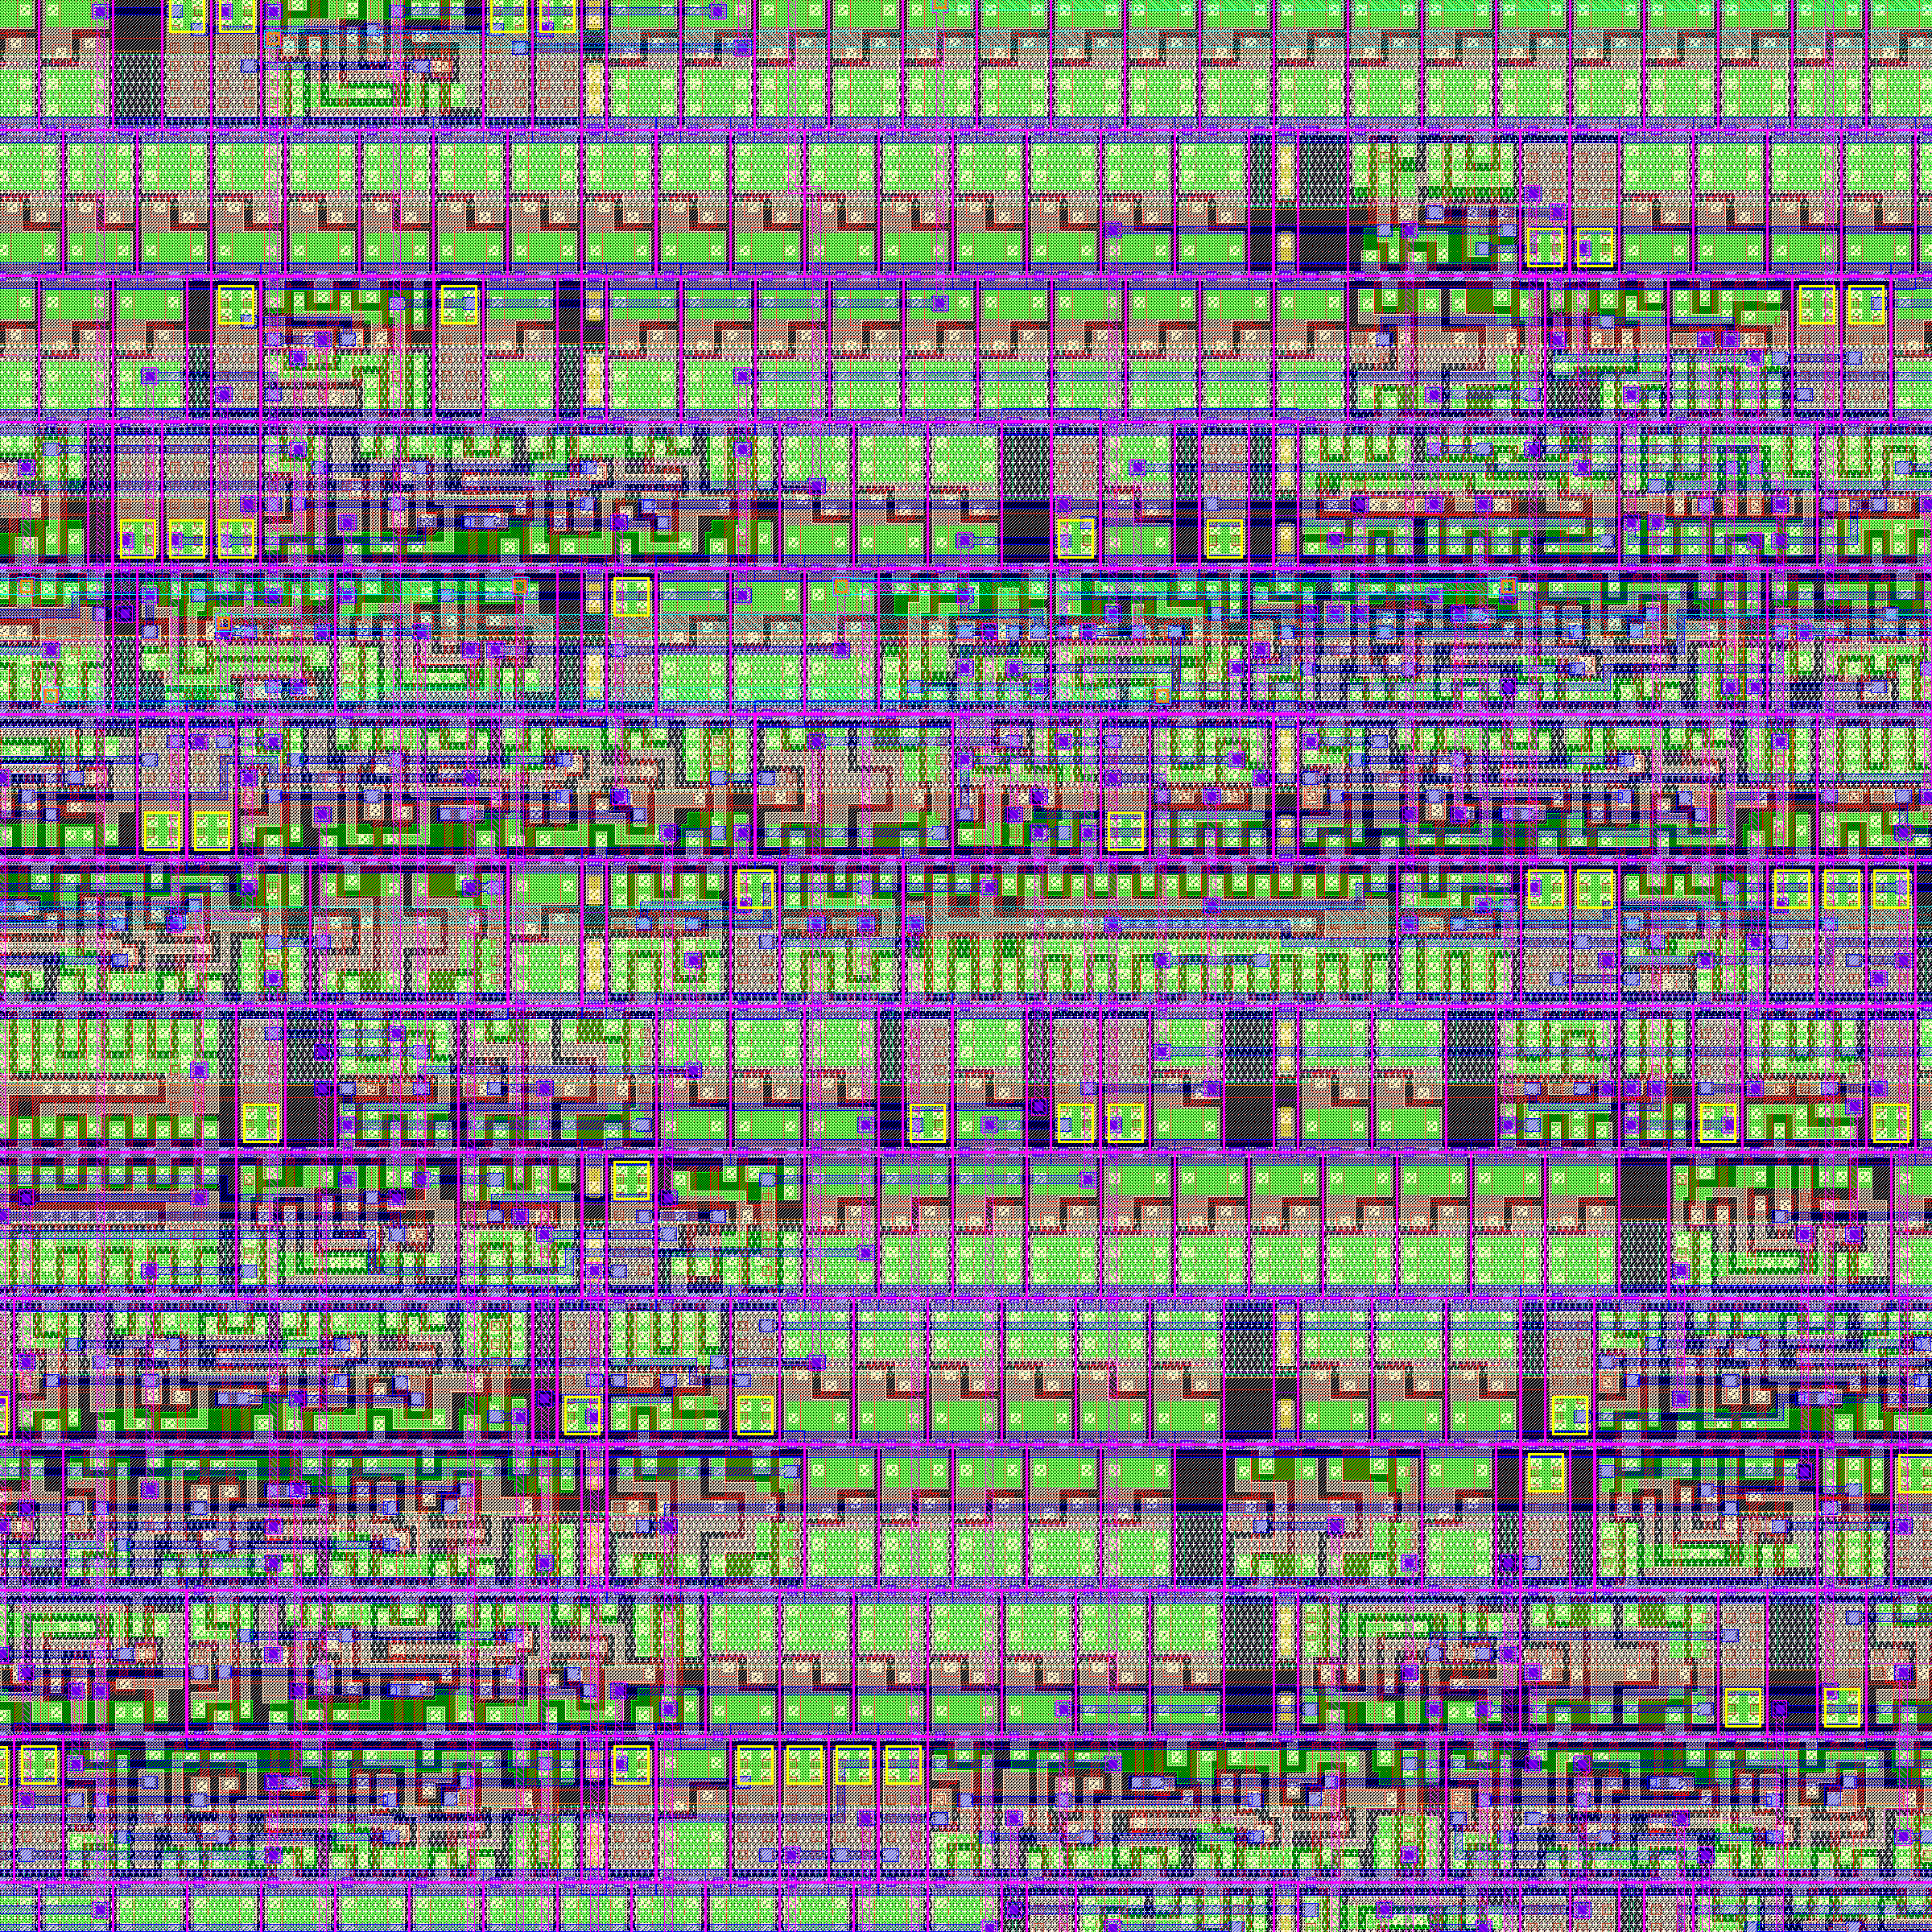
\includegraphics[width=0.45\textwidth]{images/spi_top_layout_zoom.png}\\
{\small Zoomed layout: standard-cell rows, power rails and metal routing}
\end{center}

\sect{Tools}
AMD Vivado 2024.2 XSIM and XCRG (UVM 1.2, SVA, coverage); Yosys; OpenROAD and OpenSTA; Magic; KLayout; Netgen; OpenLane~2 (LibreLane); SkyWater SKY130A PDK (\texttt{sky130\_fd\_sc\_hd}).

\sect{Conclusion}
The APB3 SPI master was taken from specification to a DRC- and LVS-clean GDSII. Verification closed with a 100\,\% pass rate, 99.8\,\% functional coverage, complete statement coverage and full toggle coverage, backed by assertion checks across all four SPI modes. The layout closes timing at 50\,MHz in all corners in 0.034\,mm$^2$ of SKY130 silicon at 1.68\,mW. All RTL, testbench, scripts, reports and the final GDS are available in the GitHub repository.

\end{document}
